\documentclass[11pt, oneside]{article} 
\usepackage{geometry}
\geometry{letterpaper} 
\usepackage{graphicx}
	
\usepackage{amssymb}
\usepackage{amsmath}
\usepackage{parskip}
\usepackage{color}
\usepackage{hyperref}

\graphicspath{{/Users/telliott_admin/Dropbox/Tex/png/}}
% \begin{center} 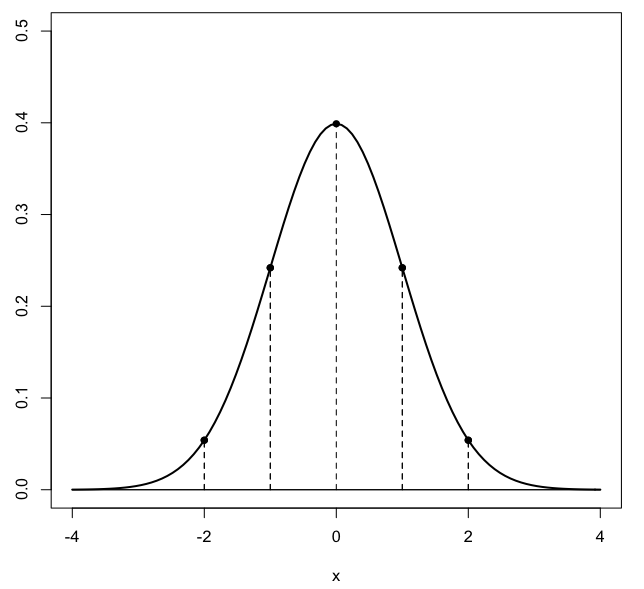
\includegraphics [scale=0.4] {gauss3.png} \end{center}

\title{Green's Theorem}
\date{}

\begin{document}
\maketitle
\Large

\label{sec:green}

We will take a look at the fundamental theorems of vector calculus.

First, though, a word about curl.  Curl measures the rotation of a vector field (its absolute value is twice the angular momentum).  As an example, if a two dimensional field $\mathbf{F}$ has components $\ \langle M,N \rangle \ $, then
\[ \text{curl} \ \mathbf{F} = N_x - M_y \]

As we'll see, the result of $\text{curl} \ \mathbf{F}$ is a vector, in this case it points out of the plane.  When we calculate with it in 2D we are implicitly forming the dot product with $\hat{\mathbf{k}}$.

Our convention is that we go on a curve around a region with $R$ on our left, then the curl points up.  This is a result of what is called the "right hand rule."

If the value of $\text{curl} \ \mathbf{F}$ is zero, then the work done going around a closed curve is also zero, alternatively if the curl is non-zero, work is done.  Think of swimming in a whirlpool.  Against the flow it is hard going, whereas with the flow, it's easy.

In our theorems, the curl will always be associated with the line integral for work.

The work done in moving along a curve $C$ is

\[ W = \int_C \mathbf{F} \cdot d\mathbf{r}  = \int_C \mathbf{F} \cdot \hat{\mathbf{T}} \ ds \]

(Normally we write the magnitude first and then the unit vector, as in $3 \mathbf{\hat{i}} + 4 \mathbf{\hat{j}}$, but here the reverse seems more natural so that the second vector comes right after the dot product).

In three dimensions, we use the "del" operator
\[ \nabla = \ \ \langle \frac{\partial}{\partial x},\frac{\partial}{\partial y},\frac{\partial}{\partial z}  \rangle \  \]

The curl of $\mathbf{F}$ is
\[ \nabla \times \mathbf{F} \]

We will write the components as $\mathbf{F} = \ \ \langle M,N,P \rangle \ $ (some authors use $\ \langle P,Q,R \rangle \ $ but I would prefer to use $M$ consistently for the $x$-component, and so on

\[ \nabla \times \mathbf{F} =  \ \ \langle P_y-N_z,M_z-P_x,N_x-M_y \rangle \  \]
which is basically impossible to remember except by using this convenient device
\[
\begin{vmatrix} 
  \hat{i}  &  \hat{j} & \hat{k} \\ 
  \frac{\partial}{\partial x}  &  \frac{\partial}{\partial y} & \frac{\partial}{\partial z} \\ 
  M  & N & P \\ 
\end{vmatrix} \ \
\]
We think of forming the "determinant" of this "matrix."

In two dimensions $P=0$ and also $M_z$ and $N_z$ are both zero, so this equation reduces to the one we saw above.

A basic fact in vector calculus is that if the field is the gradient of a potential function, the curl is zero.  Let the function be $f$ and the field $\mathbf{F} = \nabla f$, then $M=f_x$ and $N=f_y$.  Then the curl is $f_{yx}- f_{xy}$, but for any such function
\[ f_{xy} = f_{yx} \]

\subsection*{Calculating}
Let's look again at
\[ W = \int_C \mathbf{F} \cdot d\mathbf{r} = \int_C \mathbf{F} \cdot \hat{\mathbf{T}} \ ds \]
This can be written as
\[ = \int_C M \ dx + N \ dy  \]
One way to see this is to say
\[ d\mathbf{r} = \frac{d}{dt} \mathbf{r} \ dt = \ \ \langle \frac{dx}{dt},\frac{dy}{dt} \rangle \  \ dt \]
so when we do the dot product with $\mathbf{F}$, we get what is written above.

There is another important integral to be explained below
\[ \int_C \mathbf{F} \cdot \hat{\mathbf{n}} \  ds = \int_C -N \ dx + M \ dy  \]

It's really important to appreciate that although these equations look something like a double integral, they are \emph{not}.

We will have a parametrization of the curve in terms of $t$ (or $x$ or $\theta$), and a single integral like $\int_C f(t) \ dt $.

\subsection*{Green---work}
We start with two theorems in the plane (typically the $xy$-plane).  These are called Green's Theorem for work, and Green's Theorem for flux.  

Green's Theorem for work states that for a closed path

\[ \oint \mathbf{F} \cdot d\mathbf{r}  = \iint_R \ \nabla \times \mathbf{F} \ dA \]

One sticky point I had here is that the curl produces a vector, yet the formula is usually given as above.  That's because this is a special case of Stokes theorem where the term on the right is really 
\[ (\nabla \times \mathbf{F}) \cdot \hat{\mathbf{k}} \ dA \]
which (since $\nabla \times \mathbf{F} $ is parallel to $\hat{\mathbf{k}}$) gives what we have above.

Alternatively 

\[ \int_C M \ dx + N \ dy = \iint_R (N_x - M_y) \ dx \ dy \]

The work done along a closed path around $R$ is equal to the double integral over $R$ of the curl of $\mathbf{F}$.  Remember the whirlpool.

\subsection*{Green---flux}
Flux is flow across a curve, or in $\mathbb{R}^3$, through a surface.

Green's Theorem for flux (in the plane) states that for a closed path $C$ over a region $R$

\[ \int_C \mathbf{F} \cdot \hat{\mathbf{n}} \  ds = \iint_R \ \nabla \cdot \mathbf{F} \ dA \]
Alternatively
\[ \int_C M \ dy - N \ dx =  \iint_R \ (M_x + N_y) \ dx \ dy \]

Another use of the "del" operator is the divergence of $\mathbf{F}$

\[ \nabla \cdot \mathbf{F} \]
if $\mathbf{F} = \ \ \langle M,N \rangle \ $
\[ \nabla \cdot \mathbf{F} = M_x + N_y \]

The divergence of a vector field is a scalar quantity.  It measures the net production (or disappearance) of the "substance" that flows in a vector field.  If there are no sources or sinks in a region, the divergence of $\mathbf{F}$ will be zero.

Restating the theorem:

\[ \oint \mathbf{F} \cdot \hat{\mathbf{n}} \ dS  = \iint_R \ \nabla \cdot \mathbf{F} \ dA \]

Breaking this down, on the left hand side of the first version, $\hat{\mathbf{n}}$ is the unit vector \emph{orthogonal} to $\hat{\mathbf{T}}$.  Since $\hat{\mathbf{n}}$ and $\mathbf{n}$ are orthogonal to $\hat{\mathbf{T}}$ and $d\mathbf{r}$, the dot product with $\ \langle dx,dy \rangle \ $ must equal zero.  Hence, we should have

\[ \hat{\mathbf{n}} \ ds = \ \ \langle \frac{dy}{dt},-\frac{dx}{dt} \rangle \  dt \]

Another way to think about this is that we rotate by $90^{ \circ}$ clockwise.  The normal vector points to the right as we go along the curve.

\[
\begin{bmatrix} 
  \ 0  &  1 \\ 
  -1  &   0  \\ 
\end{bmatrix} \ \ 
\begin{bmatrix} 
  dx  \\ 
  dy  \\ 
\end{bmatrix} \ \ 
=
\begin{vmatrix} 
  \ \ dy  \\ 
  -dx  \\ 
\end{vmatrix} \ \ 
\]
so when we compute $\mathbf{F} \cdot \ \ \langle dy,-dx \rangle \ $ we get $\int_C M \ dy - N \ dx$.  

Looking at what we have above we can write
\[ \hat{\mathbf{n}} \ ds = \ \ \langle dy, -dx \rangle \]
Clearly $\langle dy, -dx \rangle$ is orthogonal to $\langle dx, dy \rangle$ because the dot product is zero, but what about the magnitude?  The length of the vector squared is the dot product with itself, which is $dy^2 + dx^2$ but this is just $ds^2$.  So that part works as well.

Putting it all together, then, we have
\[ \int_C \mathbf{F} \cdot \hat{\mathbf{n}} \  ds =  \iint_R \ \nabla \cdot \mathbf{F} \ dA  \]
\[ \int_C M \ dy - N \ dx =  \iint_R \ (M_x + N_y) \ dx \ dy \]

Here, the expression on the right \emph{is} a double integral.

\end{document}  